% =========================================================
% CSC311 Final Project Report Template
% Single column, 12pt, 8 pages max.
% =========================================================

\documentclass[12pt]{article}

% ---------- Packages ----------
\usepackage[margin=1in]{geometry}
\usepackage{parskip}         % blank line between paragraphs, no indent
\usepackage{graphicx}
\usepackage{booktabs}
\usepackage{amsmath, amssymb}
\usepackage{siunitx}
\usepackage[hidelinks]{hyperref}
\usepackage{caption}
\usepackage{enumitem}
\usepackage{xcolor}
\usepackage{XCharter}
\usepackage[xcharter]{newtxmath}
\usepackage[scaled=0.96]{inconsolata}

%--------- Headers and footers ------
\usepackage{fancyhdr}
\pagestyle{fancy}
\setlength{\headheight}{14.49998pt}
\fancyhf{}
\fancyhead[L]{CSC311 Project Proposal}
\fancyhead[R]{Yang, Song, Wu, Fan}
\fancyfoot[C]{\thepage}

% ---------- Captions & Lists ----------
\captionsetup{font=small, labelfont=bf}
\setlist[itemize]{noitemsep, topsep=2pt}
\setlist[enumerate]{noitemsep, topsep=2pt}

% ---------- Helpful macros ----------
\newcommand{\bestmodel}{\textit{[Best Model Name]}}
\newcommand{\projacc}{\textbf{[XX.XX\%]}}

% ---------- Safe figure helper ----------
\makeatletter
\newcommand{\maybeincludegraphics}[3]{%
  \begin{figure}[h]
    \centering
    \IfFileExists{#1}{%
      \includegraphics[width=0.7\linewidth]{#1}%
    }{%
      \fbox{%
        \parbox[c][0.28\textheight][c]{0.7\linewidth}{%
          \centering
          \vspace{0.5em}
          \textit{[Placeholder for \texttt{#1}]}\\
          Add your figure here.
          \vspace{0.5em}
        }%
      }%
    }%
    \caption{#2}
    \label{#3}
  \end{figure}%
}
\makeatother

\usepackage{xcolor}
\definecolor{royalblue}{rgb}{0.0, 0.14, 0.4}
\definecolor{royalblue(web)}{rgb}{0.25, 0.41, 0.88}
\usepackage{tcolorbox}
\tcbuselibrary{breakable}
\usepackage{comment}
\usepackage{tikz}
\usetikzlibrary{arrows.meta}


\newcommand{\vect}[1]{\mathbf{#1}}

% =========================================================
% Title Page
% =========================================================
\begin{document}

\begin{titlepage}
    \centering
    \vspace*{3cm}

    {\Large {CSC311: Introduction to Machine Learning} \par}
    \vspace{1cm}

    {\Large {Project Proposal} \par}
    \vspace{1cm}

    {\large \textit{Which Sport Is It? Predicting a Sport from Survey Answers} \par}
    \vspace{3cm}

    {\large Submitted by \par}

    \vspace{0.5cm}
    {\large Group [Number]}

    \vspace{0.5cm}
    {\large Ethan Yang, Sixuan Song, Yuzhou Wu, Zhihan Fan \par}

    \vfill
    {\large University of Toronto \\ Fall 2026 \par}
\end{titlepage}
\clearpage
\setcounter{page}{1}

% The proposal contains only the two graded sections. The Executive Summary,
% Results, and Contributions sections of the template are added for the final
% report.


% ================================================
% Data Exploration
% ================================================
\section{Data Exploration}\label{sec:data-exploration}

\textbf{Task and how the test set was set aside.} Each row is one survey response about a sport, and the label is one of three classes (\textit{Baseball}, \textit{Basketball}, \textit{Soccer}). The file has 870 rows from 290 respondents, and each respondent answered once for every sport. \emph{Before looking at any feature}, we split the respondents with a fixed seed (\texttt{split\_data.py}) into 202 for training (606 rows), 44 for validation (132 rows) and 44 for testing (132 rows). Splitting \emph{by respondent ID} keeps a person's three answers together, so a model cannot profit from recognising someone's writing style, which would not carry over to the TA/instructor test set. The ID itself is an arbitrary index and is not used as a feature. \textbf{Everything below is computed on the 606 training rows only} (\texttt{explore.py} never reads the other files). The test file is opened only once, for the final accuracy estimate. Every split is exactly one third per class (no class imbalance).

\begin{figure}[h]
\centering
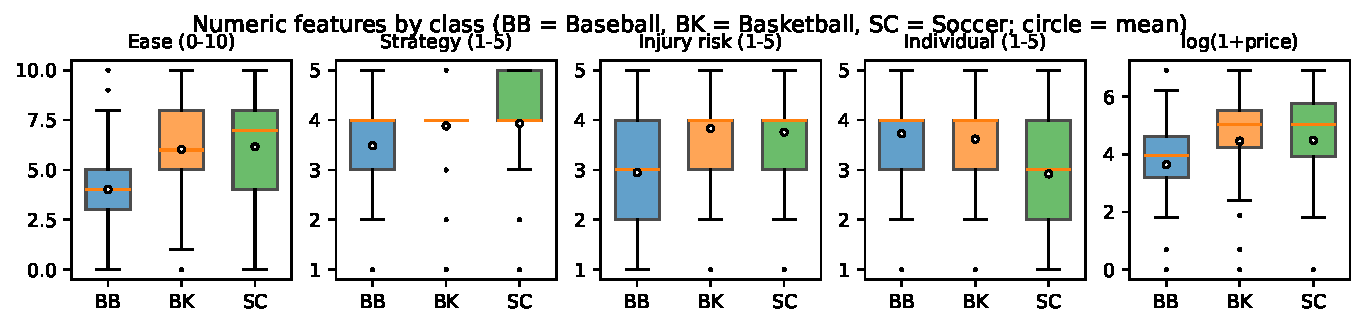
\includegraphics[width=\linewidth]{figures/numeric_by_class.pdf}\\[1pt]
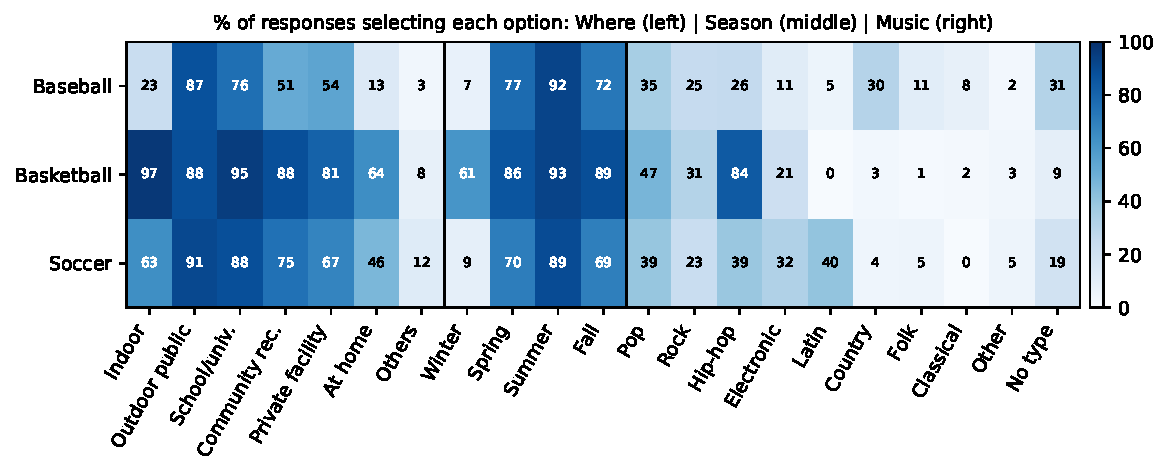
\includegraphics[width=0.74\linewidth]{figures/multiselect_by_class.pdf}
\caption{Training split only. Top: numeric features by class. Bottom: \% of each class's responses selecting each multi-select option.}\label{fig:explore}
\end{figure}

\textbf{Feature types and distributions} (Table~\ref{tab:features}). \emph{Ease} is roughly symmetric on 0--10 (mean 5.4, SD 2.4). The Likert items lean towards \emph{Agree}, and their pairwise correlations are at most $0.31$, so no pair is redundant. \emph{Price} is very right-skewed (skewness 6.7, median \$100, maximum \$5000, 13\% answered \$0). Free-text answers are short (median 1--2 words), so the encoding is sparse: 581 features for 606 rows (minimum word frequency 2), and 417 of the 564 binary features occur in under 1\% of rows. Two options are nearly constant across classes (\emph{Outdoor public space} 87--91\%, \emph{Summer} 89--93\%), so they carry little information.

\begin{table}[h]
\centering\footnotesize
\caption{Feature types, missing rate (training split) and encoding.}\label{tab:features}
\begin{tabular}{@{}llll@{}}
\toprule
Feature & Type & Missing & Encoding \\
\midrule
Ease of starting (0--10) & numeric & 0\% & median-impute, standardise \\
Strategy, Injury risk, Individual & Likert (5 levels) & 0\% & ordinal 1--5, standardise \\
Where, Season, Music & multi-select & 0\% & multi-hot (7, 4, 10 indicators) \\
Food, Colour, Song, Feeling & free text & 2.0, 0.8, 7.8, 0.0\% & binary bag-of-words per question \\
Price willing to pay & free text $\to$ \$ & 0.7\% + 2.3\% unparseable & cap \$1000, $\log(1+x)$, standardise \\
\bottomrule
\end{tabular}
\end{table}

\textbf{Missing values, outliers and inconsistencies.} All forms of empty answer (NaN, empty string, ``n/a'', ``-'') are first mapped to one missing marker. Missing rates are low, but \emph{Song} is missing for 10.9\% of Baseball and 9.9\% of Basketball rows versus 2.5\% of Soccer rows. Missingness is therefore informative, so we add a 0/1 \emph{missing} indicator for each question and impute numeric features with the training median. Answers such as ``none'' are real answers and stay as words. Text varies in case, spacing and plurals (``Hotdog'', ``hot dogs'') and contains placeholders (``[this sport]''), so our tokenizer lower-cases, drops placeholders and stop words, joins ``hot dog'' and strips plural ``s''. Price answers come in many formats (``\$1,000'', ``200CAD'', ``100-200'', ``Nothing''). We parse the number, take the midpoint of ranges and map refusals to \$0. The 2.3\% of answers with no number (``very willing'') are treated as missing. For outliers, the IQR rule flags 12\% of prices (above \$425), too many to call errors, so we cap price at \$1000 (8 answers) and take $\log(1+x)$, which reduces the skewness from 6.7 to $-1.1$. All other values are in range.

\textbf{Preprocessing and why.} \emph{Likert} items are ordinal 1--5 rather than one-hot. This keeps their order in one feature instead of five, which matters when there are about as many features as rows. \emph{Numeric} features are standardised, $x'=(x-\mu)/\sigma$, with $\mu,\sigma$ from the training rows. Gradient descent, L2 penalties and neural networks are scale-sensitive. \emph{Multi-select} answers become multi-hot 0/1 vectors, since several options can be chosen. \emph{Free text} becomes a binary bag-of-words with a separate vocabulary for each question. We use presence rather than counts because answers are 1--2 words long. Words seen fewer than \texttt{min\_df} times in training are dropped, and words first seen at prediction time are ignored. \texttt{min\_df} and binary vs.\ TF-IDF weighting are tuned (Section~\ref{sec:methodology}). Every learned quantity (medians, $\mu,\sigma$, vocabularies) is fitted on training data only (\texttt{preprocess.py}).

\textbf{Which features are predictive.} We compare the gap between class means with the within-class SD, and compute each feature's mutual information (MI) with the label. \emph{Ease} separates Baseball (mean 4.0) from Basketball/Soccer (6.0/6.2), with gap/SD $=1.0$. Baseball also scores lower on \emph{injury risk} (2.95 vs.\ 3.8), and Soccer scores lower on \emph{individual brilliance} (2.9 vs.\ 3.6). \emph{Strategy} and \emph{price} are weak (gap/SD $<0.5$). In Fig.~\ref{fig:explore}, several options pick out one class: \emph{Indoor} (23/97/63\% for Baseball/Basketball/Soccer), \emph{Winter} (61\% for Basketball, under 10\% otherwise), \emph{Hip-hop} (84\% Basketball), \emph{Latin} (40\% Soccer) and \emph{Country} (30\% Baseball). The strongest single features are words used almost only for one class: ``waka''/``shakira'' (100\% Soccer), ``take me out to the ball game'' ($\ge$95\% Baseball), ``green'' (95\% Soccer), ``orange'' (95\% Basketball) and ``peanut'' (93\% Baseball). The highest MI is for \texttt{song:waka}, \texttt{where=Indoor} and \texttt{colour:green} (0.31--0.32 bits). \textbf{Implications:} many sparse indicators, each adding some evidence for one class, suit a regularised linear model; threshold effects and interactions (indoor \emph{and} winter) suit tree ensembles; with $p\approx n$, all models need strong regularisation.

% ================================================
% Methodology
% ================================================
\section{Planned Methodology}\label{sec:methodology}

\textbf{Model families.} Each family is motivated by Section~\ref{sec:data-exploration}, and each can be re-implemented with numpy alone in \texttt{pred.py}.
\begin{enumerate}[leftmargin=*]
\item \textbf{Softmax (multinomial logistic) regression with L2.} Most features are sparse indicators, and each adds a small, roughly independent amount of evidence for one class. That is exactly the additive log-odds model that softmax regression assumes. It has the lowest variance of our candidates, which matters with 581 features and 606 rows, and its weights are interpretable.
\item \textbf{Random forest} \cite{breiman2001rf}. Several effects are threshold-shaped (Baseball if ease $\le 4$, Basketball if \emph{Winter}) and may interact. Trees capture both without scaling and are unaffected by the remaining skew. Averaging many decorrelated trees removes most of a single tree's variance.
\item \textbf{Multilayer perceptron (MLP).} Hidden units can learn non-linear combinations of features (e.g.\ a word that matters only together with a season). With L2 regularisation and early stopping, it is a flexible middle ground between the two models above.
\end{enumerate}
We decided not to use $k$-nearest neighbours: in 581 mostly-zero dimensions, distances are dominated by irrelevant word features (the curse of dimensionality), and untuned $k$NN was clearly worse in our preliminary check (Table~\ref{tab:prelim}). We also ruled out fine-tuning a language model, because 606 rows are too few and \texttt{pred.py} may only use numpy and pandas.

\textbf{Training setup.} Let $\vect{x}^{(i)}\in\mathbb{R}^{D}$ be an encoded response with label $y^{(i)}\in\{1,2,3\}$. Models are trained with scikit-learn 1.9 \cite{pedregosa2011sklearn} on top of our own \texttt{preprocess.py}, and every random seed is fixed to 311.
\begin{itemize}[leftmargin=*]
\item \emph{Softmax regression:} $\vect{z}=\vect{W}\vect{x}+\vect{b}$ and $p(y=k\mid\vect{x})=e^{z_k}/\sum_j e^{z_j}$. We minimise $\frac1N\sum_i -\log p(y^{(i)}\mid\vect{x}^{(i)})+\frac{\lambda}{2}\lVert\vect{W}\rVert_F^2$, where $C=1/(\lambda N)$. The objective is convex, so we use L-BFGS (tolerance $10^{-4}$, at most 2000 iterations), and every run reaches the same optimum.
\item \emph{Random forest:} Gini impurity and bootstrap samples. Trees are grown greedily, so there is no gradient optimiser. Regularisation comes from \texttt{max\_depth}, \texttt{min\_samples\_leaf} and \texttt{max\_features}.
\item \emph{MLP:} ReLU hidden layers, a softmax output and the cross-entropy loss. We use Adam ($\beta_1=0.9$, $\beta_2=0.999$) with mini-batches of 32, a constant learning rate $\eta$ and an L2 penalty $\alpha$. Early stopping is done by tuning the number of epochs with grouped CV. We do not use scikit-learn's built-in early stopping, because its internal split is random by row and can put the same respondent on both sides.
\end{itemize}

\textbf{Validation scheme.} (1) \emph{Tuning:} 5-fold \textbf{grouped} cross-validation (\texttt{GroupKFold} on respondent ID) on the 606 training rows. The \texttt{FeatureBuilder} is re-fitted inside every fold, so the vocabulary, medians and $\mu,\sigma$ never see the held-out fold. (2) \emph{Model selection:} each family is refit on all training rows with its best hyperparameters and scored once on the 132 validation rows, and the highest validation macro-F1 wins. (3) \emph{Final estimate:} the chosen model is trained on training\,+\,validation and scored once on the 132 test rows, which gives our single-number test estimate. Only after that do we retrain on all 870 rows for \texttt{pred.py}.

\textbf{Hyperparameter search} (Table~\ref{tab:hparams}). Scale parameters ($C$, $\alpha$, $\eta$) are searched on log-spaced values. Each range goes from clear underfitting ($C=10^{-3}$, depth 3) to clear overfitting ($C=10^{2}$, unlimited depth). If the best value is at the edge of a range, we extend the range and search again. Softmax regression uses a full grid of 88 settings, and the forest and the MLP each use 60 random-search settings, so all three families get a similar budget. Settings are compared by mean grouped-CV macro-F1, with accuracy as the tie-breaker. If two settings are within one standard error, we pick the simpler one. To show that the ranges are reasonable, we will plot validation curves (CV score against $C$, \texttt{max\_depth} and $\alpha$) with the peak inside each range. \textbf{All three families are fully tuned before they are compared.} Tuning only the winner would be unfair to the others.

\begin{table}[h]
\centering\footnotesize
\caption{Planned search, grouped 5-fold CV on the training split. Shared by all models: \texttt{min\_df} $\in\{1,2,3,5\}$, text weighting $\in\{$binary, TF-IDF$\}$.}\label{tab:hparams}
\begin{tabular}{@{}lll@{}}
\toprule
Model (search) & Hyperparameter & Values tried \\
\midrule
Softmax regression (full grid, 88) & $C = 1/(\lambda N)$ & 11 log-spaced values, $10^{-3}$ to $10^{2}$ \\
\midrule
Random forest (random, 60) & \texttt{n\_estimators}; \texttt{max\_depth} & $\{100, 300, 600\}$; $\{3, 5, 10, 20, \text{None}\}$ \\
 & \texttt{min\_samples\_leaf}; \texttt{max\_features} & $\{1, 2, 5, 10\}$; $\{\sqrt{D},\ \log_2 D,\ 0.1D,\ 0.3D\}$ \\
\midrule
MLP (random, 60; 3 seeds each) & hidden layers; L2 penalty $\alpha$ & $(32), (64), (128), (64,32)$; log-uniform $[10^{-5}, 1]$ \\
 & learning rate $\eta$ & $\{10^{-4}, 3\!\times\!10^{-4}, 10^{-3}, 3\!\times\!10^{-3}\}$ \\
 & epochs (early stopping) & $\{25, 50, 100, 200, 400\}$ \\
\bottomrule
\end{tabular}
\end{table}

\textbf{Evaluation metrics.} For class $k$, $\text{P}_k=\frac{\text{TP}_k}{\text{TP}_k+\text{FP}_k}$, $\text{R}_k=\frac{\text{TP}_k}{\text{TP}_k+\text{FN}_k}$ and $\text{F1}_k=\frac{2\text{P}_k\text{R}_k}{\text{P}_k+\text{R}_k}$.
\begin{itemize}[leftmargin=*]
\item \textbf{Accuracy:} \texttt{pred.py} is graded on test accuracy, and our classes are balanced, so it is a meaningful headline number.
\item \textbf{Macro-F1} $=\frac13\sum_k\text{F1}_k$ (the selection metric) weights every sport equally and drops sharply when a model neglects one class. For example, always predicting one class gives 33\% accuracy but only 0.17 macro-F1. The TA-written test set may differ from ours in class mix and wording, so we want a model that does well on all three sports. We prefer macro- over weighted-averaging because no sport matters more than another.
\item \textbf{Per-class precision/recall and the confusion matrix} show which sports get confused. We expect Basketball vs.\ Soccer, whose \emph{ease} and \emph{injury} distributions overlap (Fig.~\ref{fig:explore}).
\item \textbf{Mean $\pm$ SD over the 5 folds}, so that we do not over-interpret differences smaller than the fold-to-fold noise.
\end{itemize}

\textbf{Preliminary check.} To make sure the pipeline works, we ran each family with default settings through the same grouped CV on the training split (\texttt{preliminary\_check.py}). These numbers are \emph{untuned} and are not results.

\begin{table}[h]
\centering\footnotesize
\caption{Untuned grouped 5-fold CV on the training split (606 rows).}\label{tab:prelim}
\begin{tabular}{@{}lcc@{}}
\toprule
Model (default settings) & Accuracy (mean $\pm$ SD) & Macro-F1 \\
\midrule
Majority-class baseline & $0.333 \pm 0.000$ & 0.167 \\
Softmax regression ($C=1$) & $0.914 \pm 0.022$ & 0.914 \\
Random forest (300 trees) & $0.917 \pm 0.024$ & 0.917 \\
MLP (64 hidden units, $\alpha=10^{-3}$) & $0.899 \pm 0.013$ & 0.900 \\
$k$NN ($k=15$) & $0.837 \pm 0.021$ & 0.833 \\
\bottomrule
\end{tabular}
\end{table}

\textbf{Additional analyses.} (i) A \emph{feature-group ablation} that drops song, colour, food, feeling or the multi-select group in turn. TAs may name different songs, so we want to know how much we rely on a few strong words. (ii) A \emph{soft-voting ensemble} of the three tuned models, evaluated with the same protocol. (iii) One-hot vs.\ ordinal Likert encoding, and word bigrams, both tested inside the same CV loop.

% ==================================================
% References
% ==================================================
\renewcommand{\refname}{References}
\bibliographystyle{plain}
\bibliography{references}

\end{document}
